
\documentclass[border=8pt, multi, tikz]{standalone} 
\usepackage{import}
\subimport{../layers/}{init}
\usetikzlibrary{positioning}
\usetikzlibrary{3d} %for including external image 

\def\ConvColor{rgb:yellow,5;red,2.5;white,5}
\def\ConvReluColor{rgb:yellow,5;red,5;white,5}
\def\PoolColor{rgb:red,1;black,0.3}
\def\UnpoolColor{rgb:blue,2;green,1;black,0.3}
\def\FcColor{rgb:blue,5;red,2.5;white,5}
\def\FcReluColor{rgb:blue,5;red,5;white,4}
\def\SoftmaxColor{rgb:magenta,5;black,7}   
\def\SumColor{rgb:blue,5;green,15}

\newcommand{\copymidarrow}{\tikz \draw[-Stealth,line width=0.8mm,draw={rgb:blue,4;red,1;green,1;black,3}] (-0.3,0) -- ++(0.3,0);}

\begin{document}
\begin{tikzpicture}
\tikzstyle{connection}=[ultra thick,every node/.style={sloped,allow upside down},draw=\edgecolor,opacity=0.7]
\tikzstyle{copyconnection}=[ultra thick,every node/.style={sloped,allow upside down},draw={rgb:blue,4;red,1;green,1;black,3},opacity=0.7]

\node[canvas is zy plane at x=0] (input0) at (-3,0,0) {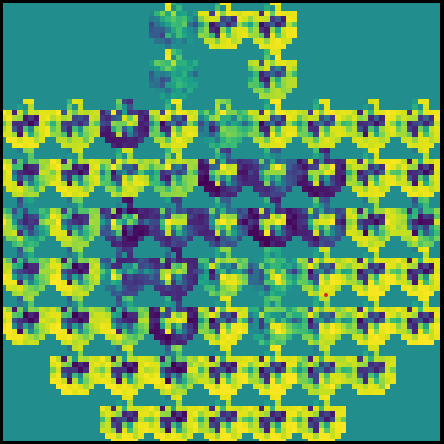
\includegraphics[width=6cm,height=6cm]{sfcc.png}};

\node[canvas is zy plane at x=0] (input1) at (-2.75,0,0) {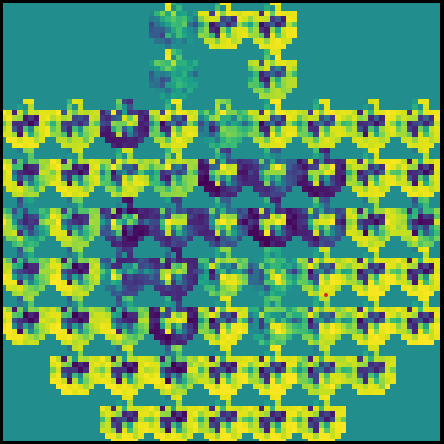
\includegraphics[width=6cm,height=6cm]{sfcc.png}};

\node[canvas is zy plane at x=0] (input2) at (-2.5,0,0) {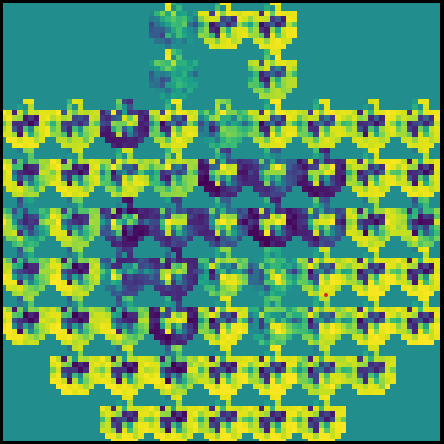
\includegraphics[width=6cm,height=6cm]{sfcc.png}};

\pic[shift={(0,0,0)}] at (0,0,0) 
    {Box={
        name=conv1,
        caption=Conv1
32@3x3,
        xlabel={{32, }},
        zlabel=81,
        fill=\ConvColor,
        height=27,
        width=12,
        depth=27
        }
    };

\pic[shift={ (2,0,0) }] at (conv1-east) 
    {Box={
        name=pool1,
        caption=MaxPool
3x3,
        xlabel={{32, }},
        zlabel=27,
        fill=\PoolColor,
        opacity=0.5,
        height=9,
        width=12,
        depth=9
        }
    };

\pic[shift={(1.5,0,0)}] at (pool1-east) 
    {Box={
        name=conv2,
        caption=Conv2
64@3x3,
        xlabel={{64, }},
        zlabel=27,
        fill=\ConvColor,
        height=9,
        width=12,
        depth=9
        }
    };

\pic[shift={ (1.5,0,0) }] at (conv2-east) 
    {Box={
        name=pool2,
        caption=Global
Max Pool,
        xlabel={{64, }},
        zlabel=1,
        fill=\PoolColor,
        opacity=0.5,
        height=1,
        width=12,
        depth=1
        }
    };

\pic[shift={(2,0,0)}] at (pool2-east) 
    {Box={
        name=fc1,
        caption=FC1 (64),
        xlabel={{" ","dummy"}},
        zlabel=64,
        fill=\SoftmaxColor,
        opacity=0.8,
        height=1,
        width=1,
        depth=16
        }
    };

\pic[shift={(1,0,0)}] at (fc1-east) 
    {Box={
        name=fc2,
        caption=FC2 (32),
        xlabel={{" ","dummy"}},
        zlabel=32,
        fill=\SoftmaxColor,
        opacity=0.8,
        height=1,
        width=1,
        depth=8
        }
    };

\pic[shift={(1,0,0)}] at (fc2-east) 
    {Box={
        name=fc3,
        caption=FC3 (3),
        xlabel={{" ","dummy"}},
        zlabel=3,
        fill=\SoftmaxColor,
        opacity=0.8,
        height=1,
        width=1,
        depth=3
        }
    };

\draw [connection]  (conv1-east)    -- node {\midarrow} (pool1-west);

\draw [connection]  (pool1-east)    -- node {\midarrow} (conv2-west);

\draw [connection]  (conv2-east)    -- node {\midarrow} (pool2-west);

\draw [connection]  (pool2-east)    -- node {\midarrow} (fc1-west);

\end{tikzpicture}
\end{document}
